\chapter{Further experiments}
\label{ch:further}
In this chapter we show some extra experimental results achieved with the system proposed in this thesis.
In particular, we show a practical application of our system to a real-world problem. 
\subsection{MEP: Maps for Easy Path}
In everyday life almost everyone owns a mobile smartphone, equipped with a camera, GPS, IMU and magnetometer sensors. 
These devices opens new possibilities for veried applications.
Maps for Easy Path aims at supporting people endowed by a simple mobile smartphone to navigate through an environment following the easiest path, \ie, the path with less irregularities in the road surface. 
Two aspects concur to the definition of a ``good'' path.
A first aspect is the history of the paths the users cover, assumes that most people tends to travel on a practical path; this involve to estimate the trajectory of the users by fusing together the data from smartphone sensors. 
The second way to help the people to define a good path is to provide a tool to notify the MEP system, that a certain  region of the environment is unfeasible or in bad condition.

We developed the latter point through the techniques defined in the previous chapter.
To notify which part of the environment presents some issue, first we need to build a map of the environment itself. 
We processed the sequence of the images acquired by a user which walked around the environment, through the OpenMVG Structure from Motion software. 
We built the rough mesh of the environment as described in Chapter \ref{ch:manif} and we refined it with the photometric procedure described in Section \ref{sec:Incremental_photoconsistent}

After the map is available, we are able to localize  camera  of the user who is going to notify the issue.
First, we have a rough position from GPS of the smartphone. 
Then we look for the images used to build the map which are in the neighborhood of this GPS location.
Now we compare these images to the query image in order to find the closest one. 
The comparison have been accomplished by detecting describing  and matching corresponding features in the images; after a RANSAC filtering on the epipolar constraint, we consider the image with the highest number of good matches as the initial guess for the query image positioning.
Finally, we refine the smartphone camera pose. 
Since we know 2D to 2D correspondence between the query and the closest images, and we know the pose of the closest images, we project its 2D features to the 3D map of the environment, then we estimate the query position though the iterative PnP algorithm \cite{hartley2003multiple} robusifyed with RANSAC.




\begin{figure}[t]
\centering
\setlength{\tabcolsep}{1px}
\begin{tabular}{ccc}
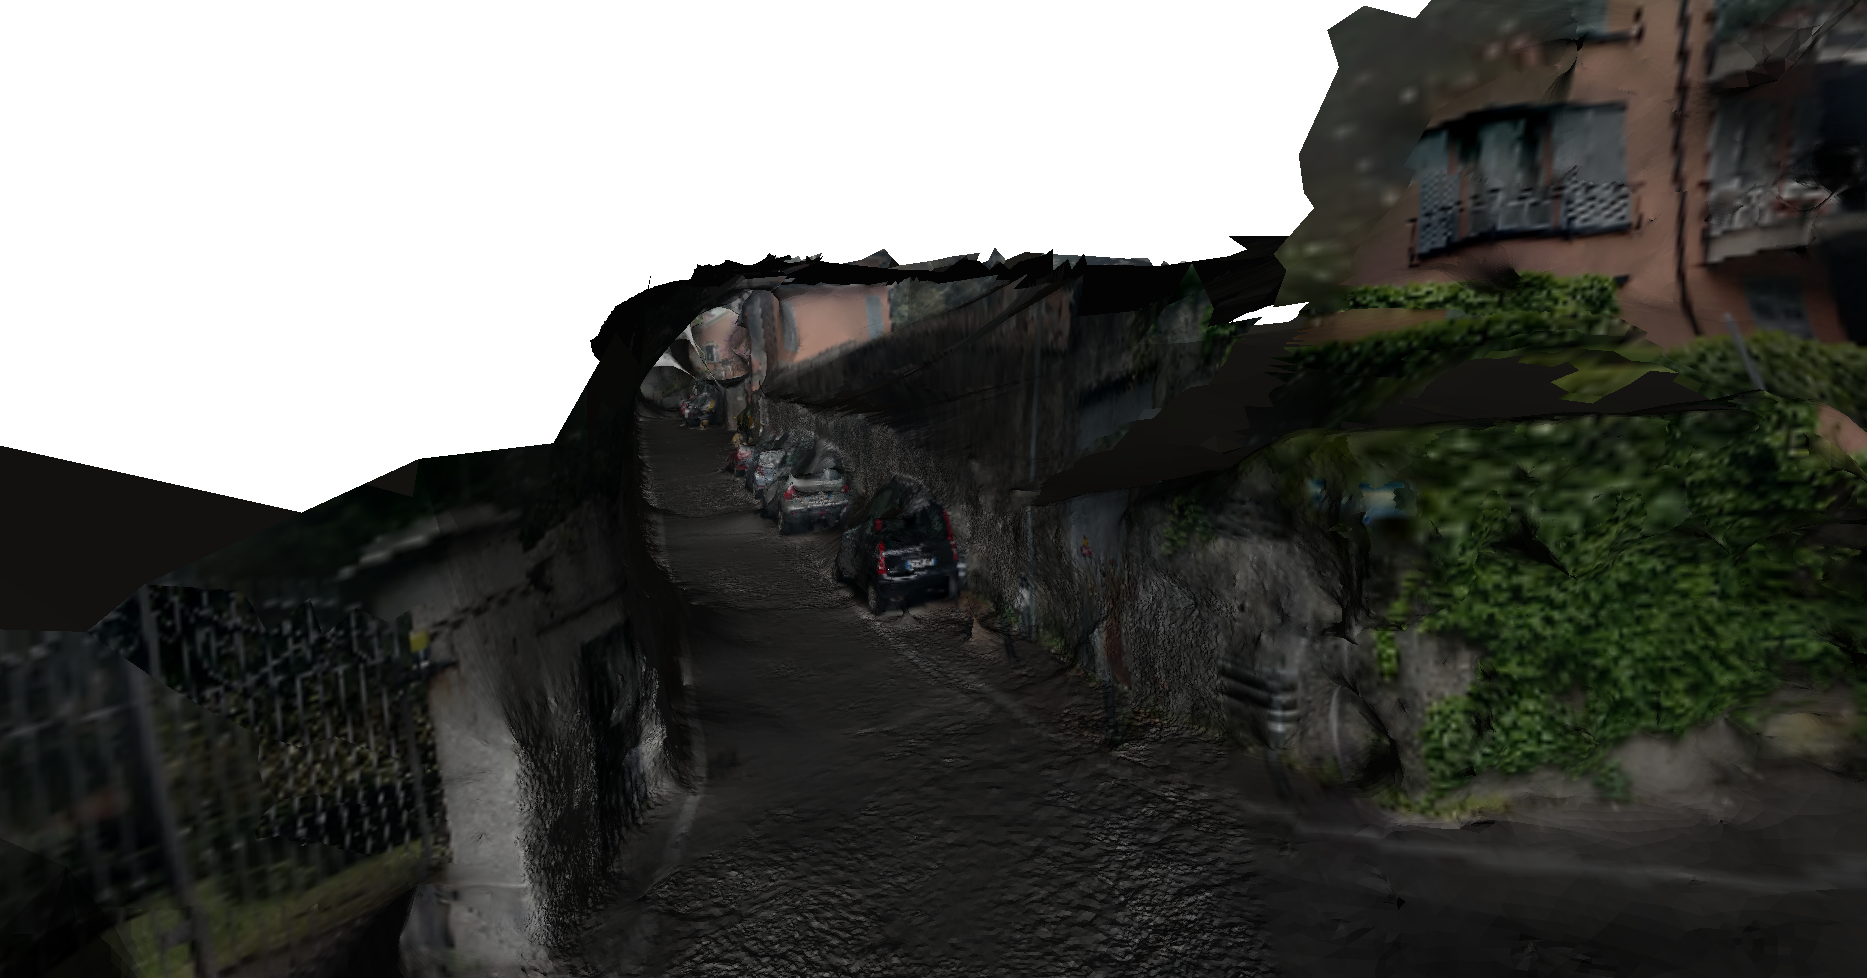
\includegraphics[width=0.325\textwidth]{./img/ch-further/18_b0100}&
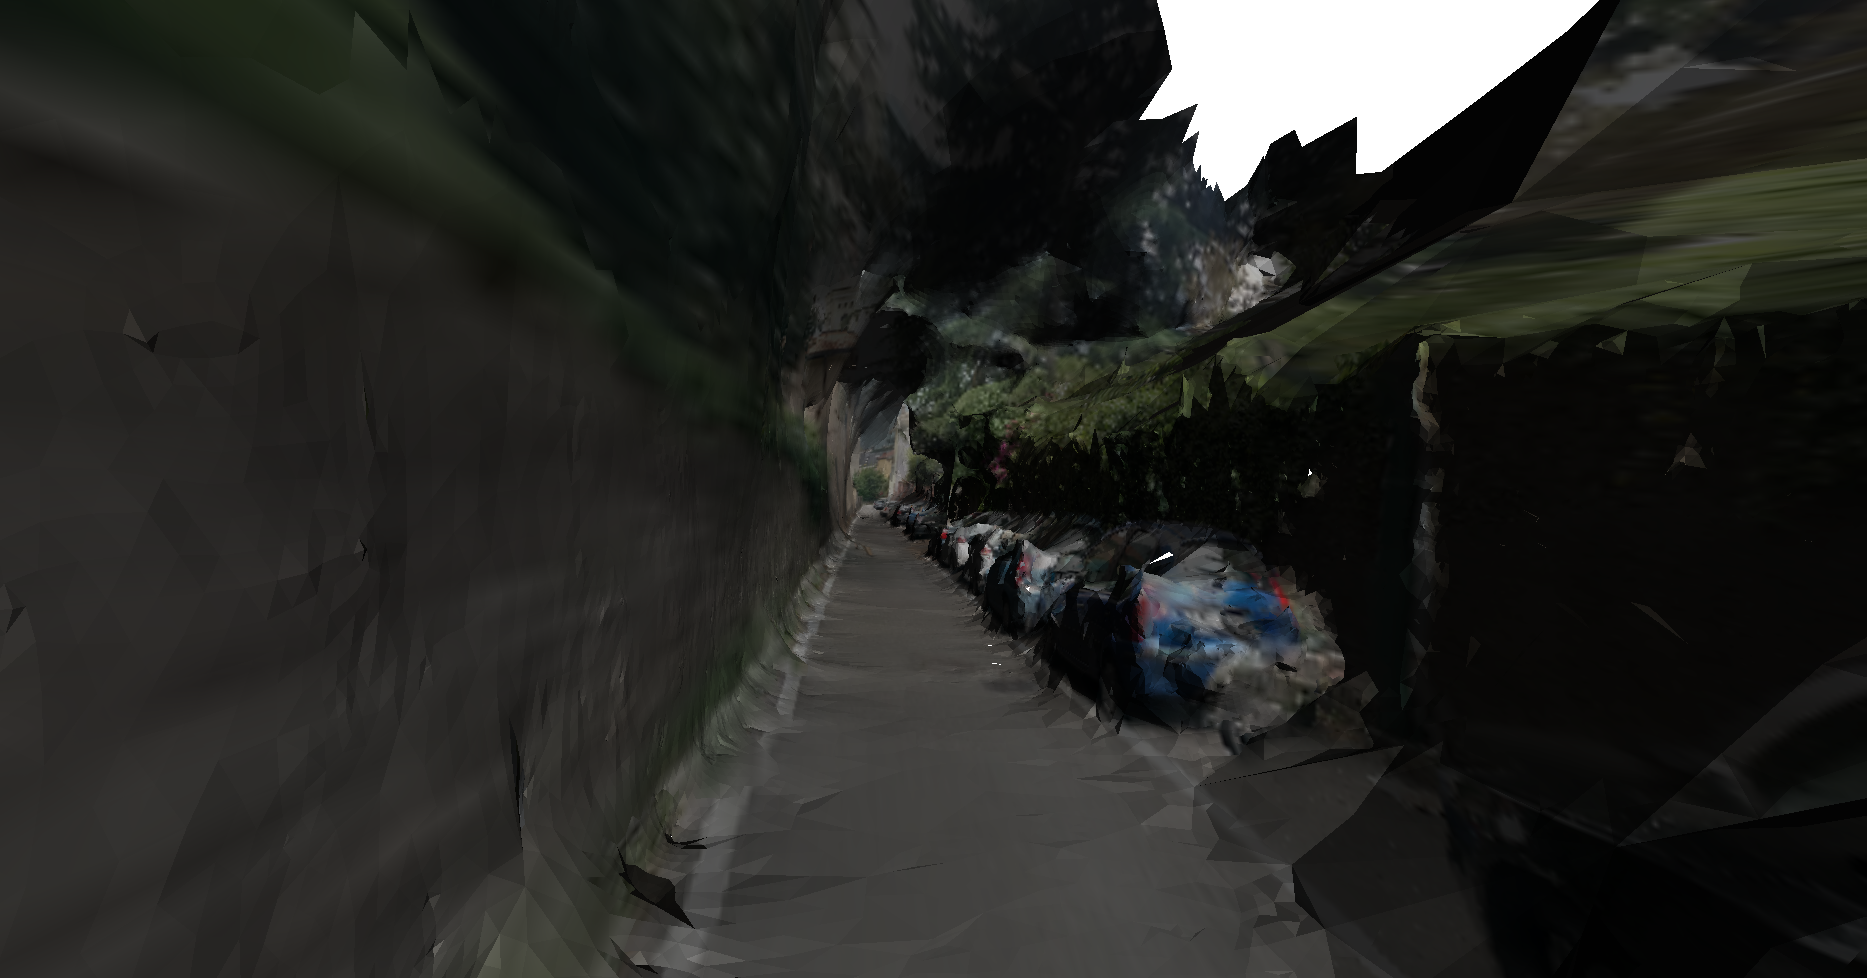
\includegraphics[width=0.325\textwidth]{./img/ch-further/18_b0101}&
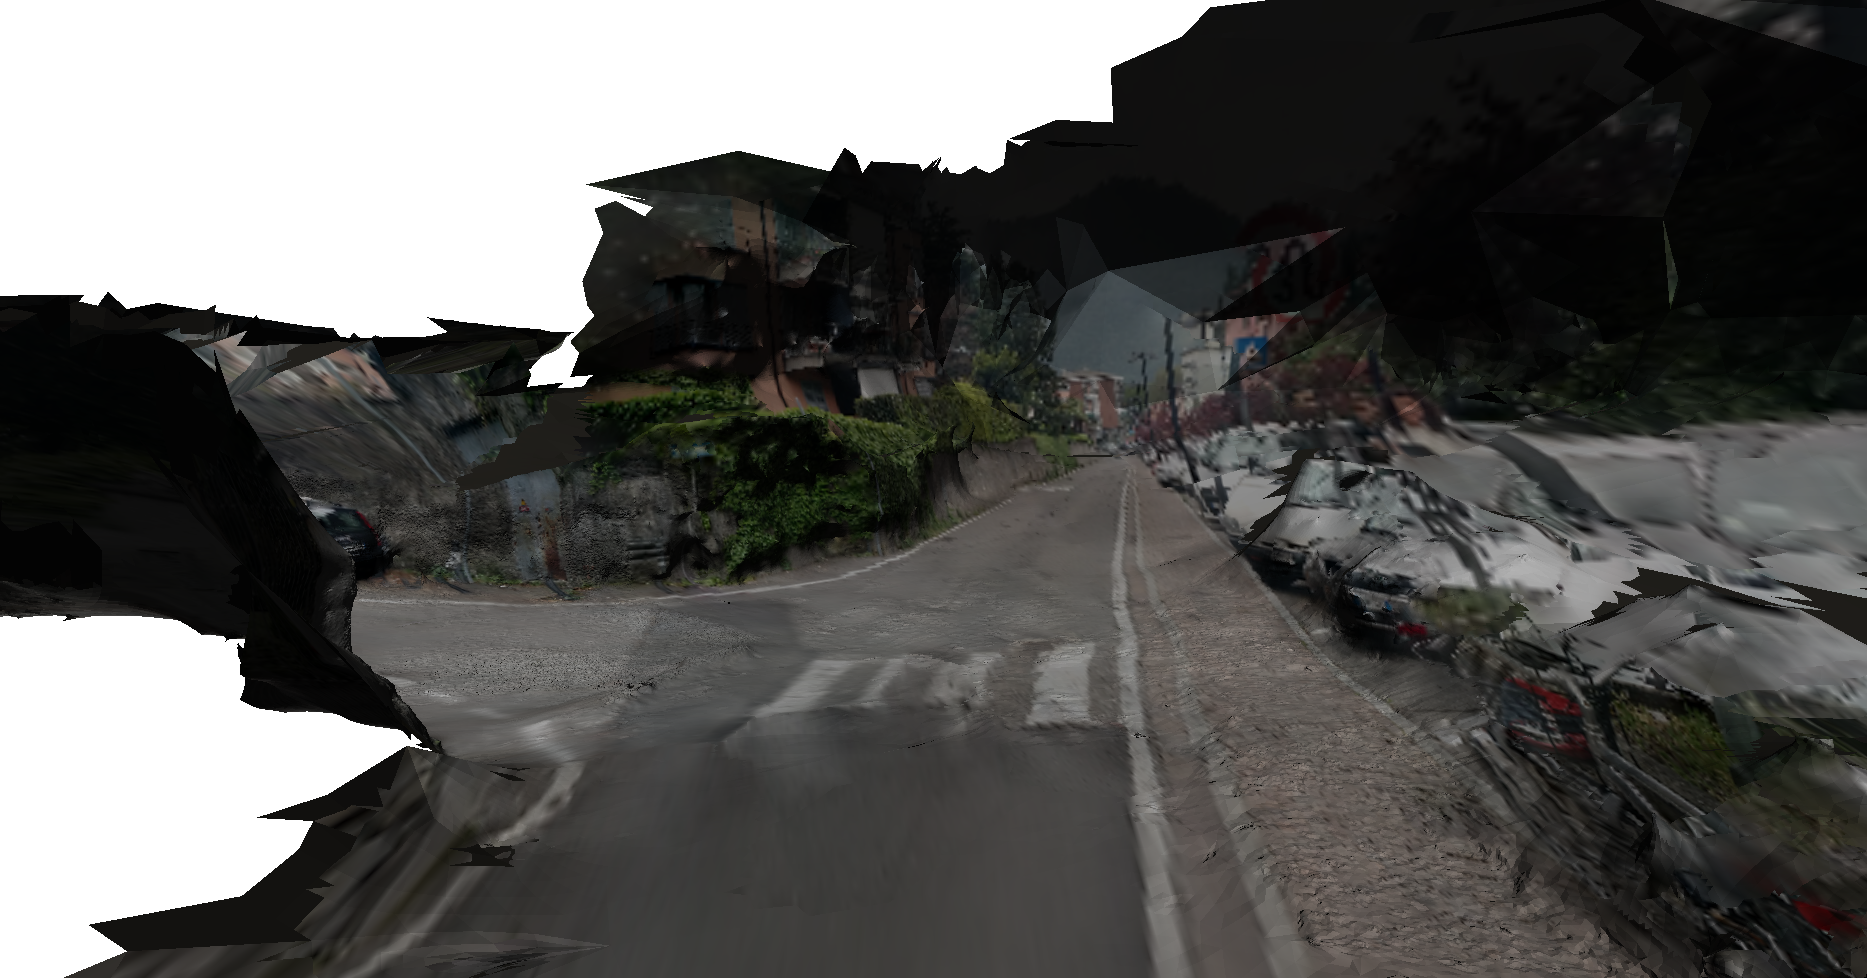
\includegraphics[width=0.325\textwidth]{./img/ch-further/18_b0102}\\
\multicolumn{3}{c}{Sequence 1}\\
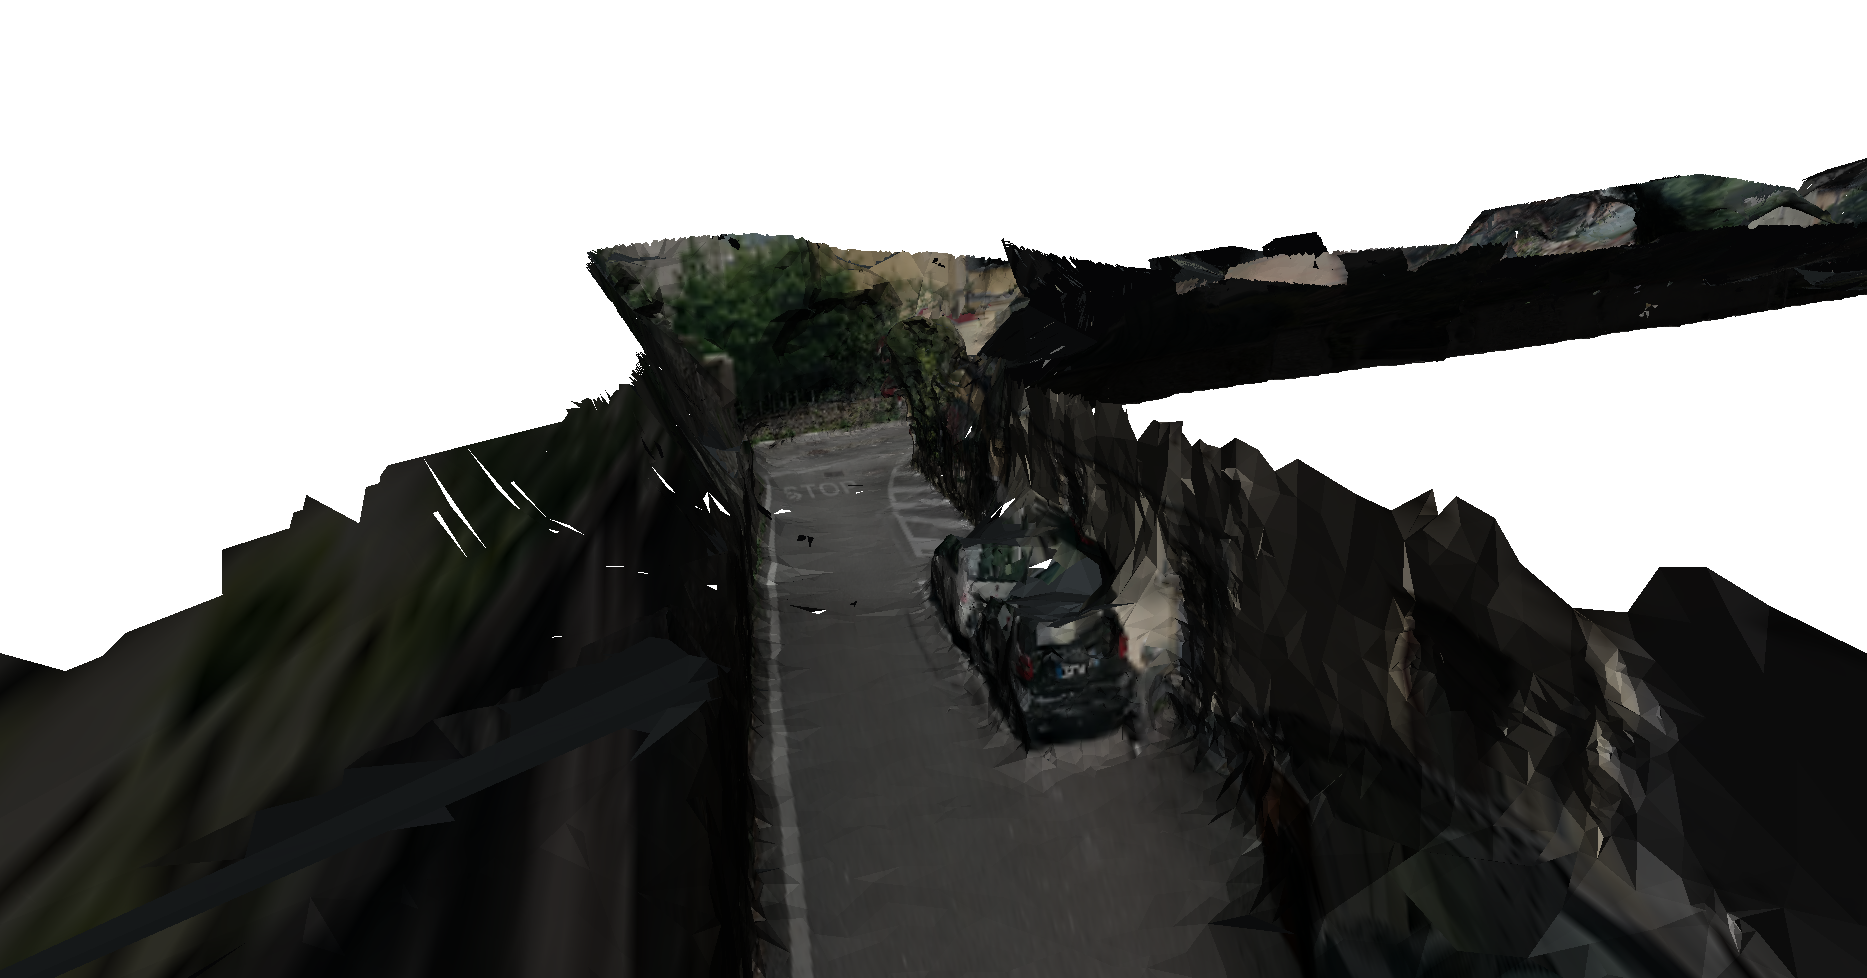
\includegraphics[width=0.325\textwidth]{./img/ch-further/18_c00}&
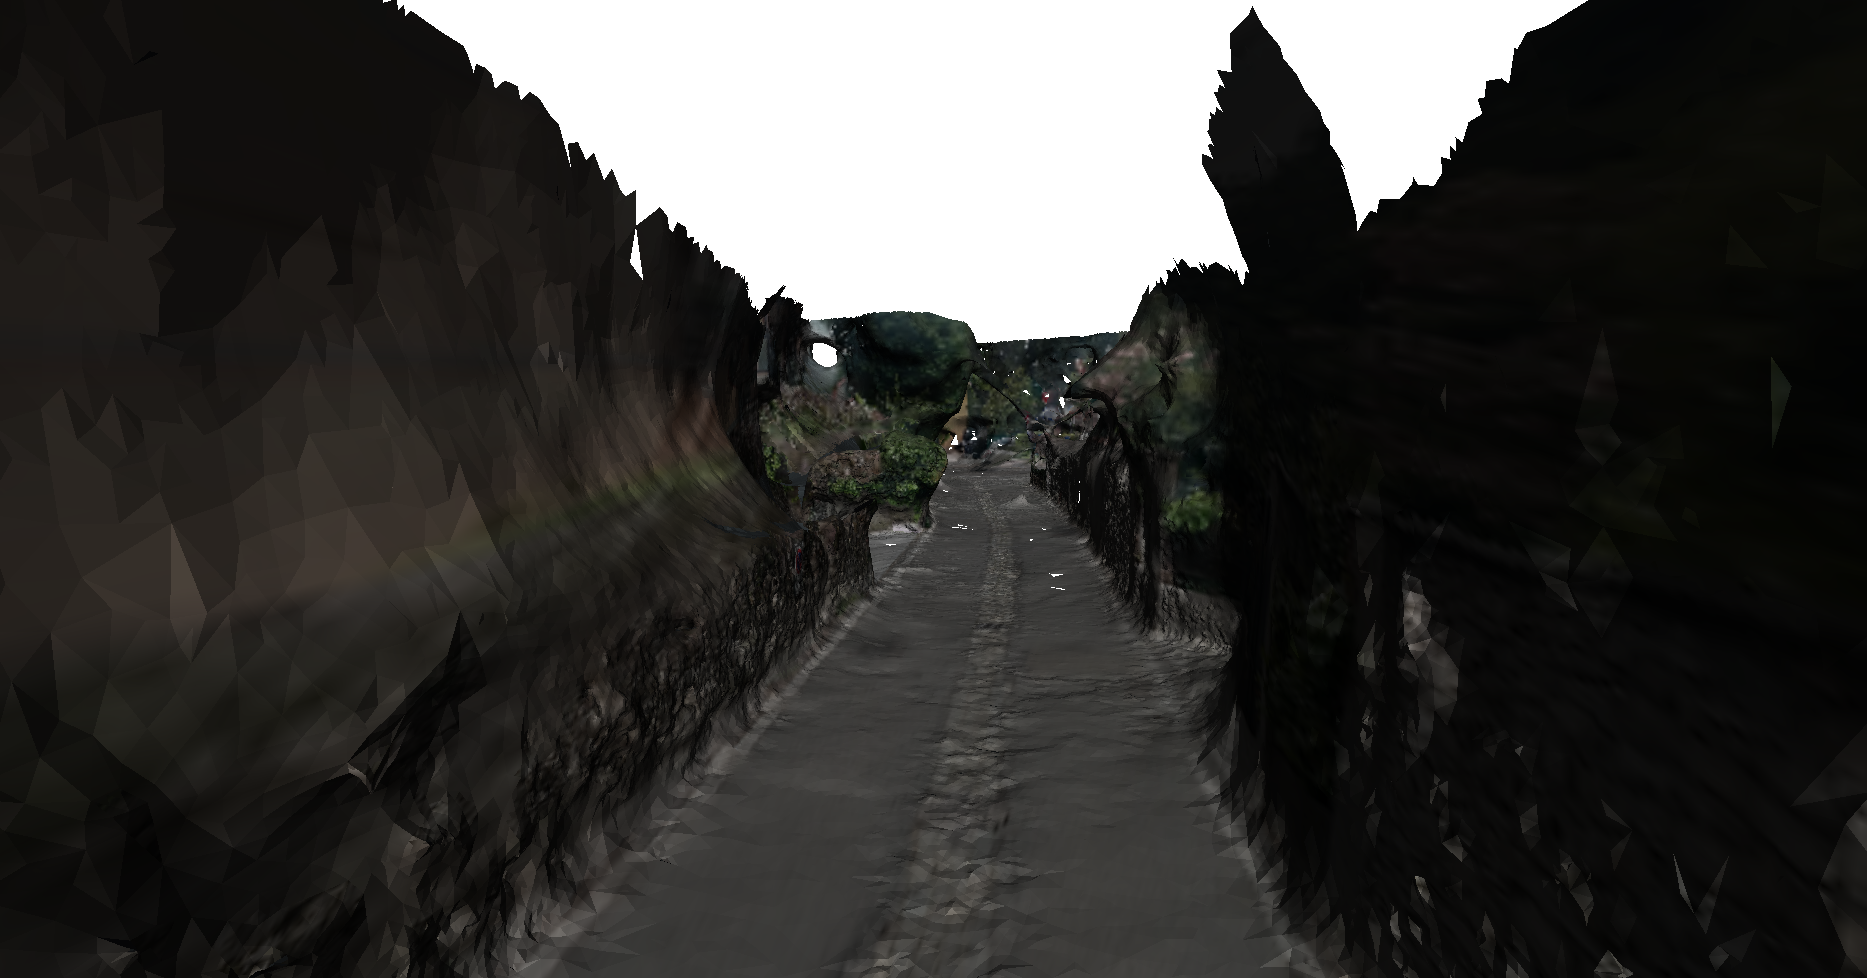
\includegraphics[width=0.325\textwidth]{./img/ch-further/18_c02}&
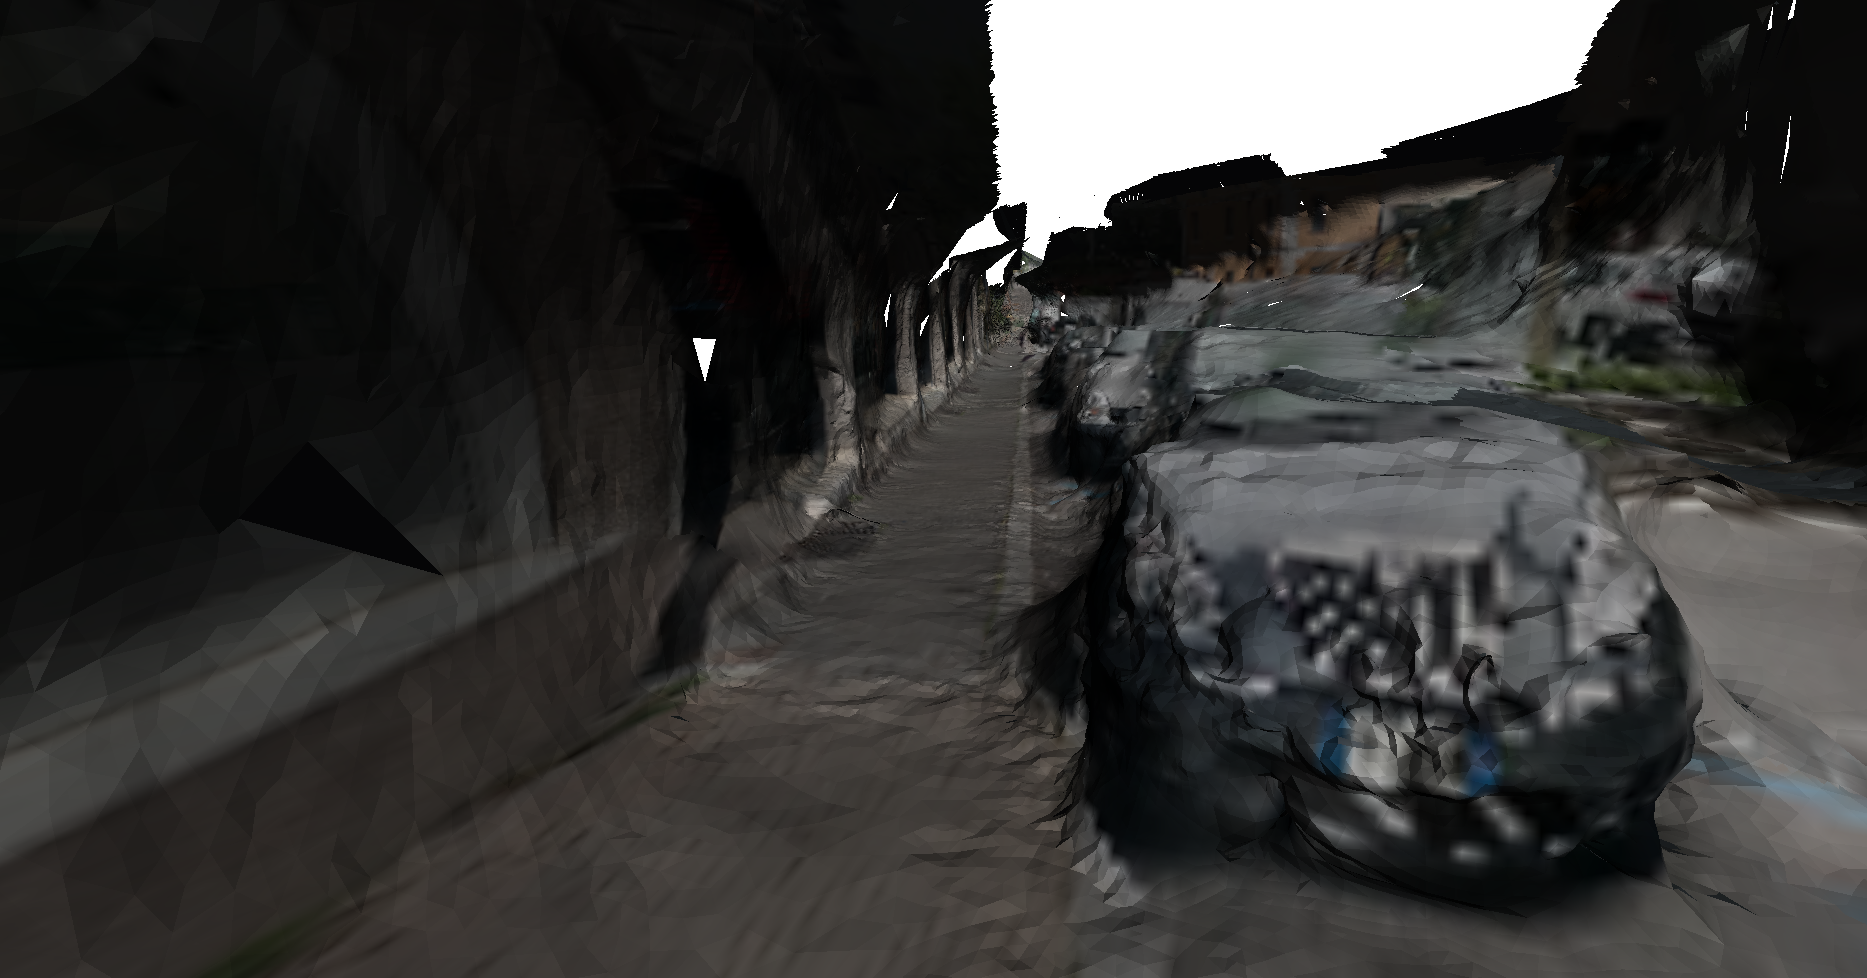
\includegraphics[width=0.325\textwidth]{./img/ch-further/18_c04}\\
\multicolumn{3}{c}{Sequence 2}\\
\end{tabular}
\caption{Example of (textured) reconstructions}
\label{fig:mep_reconstr}
\end{figure}



\begin{figure}[t]
\centering
\setlength{\tabcolsep}{1px}
\begin{tabular}{cc}
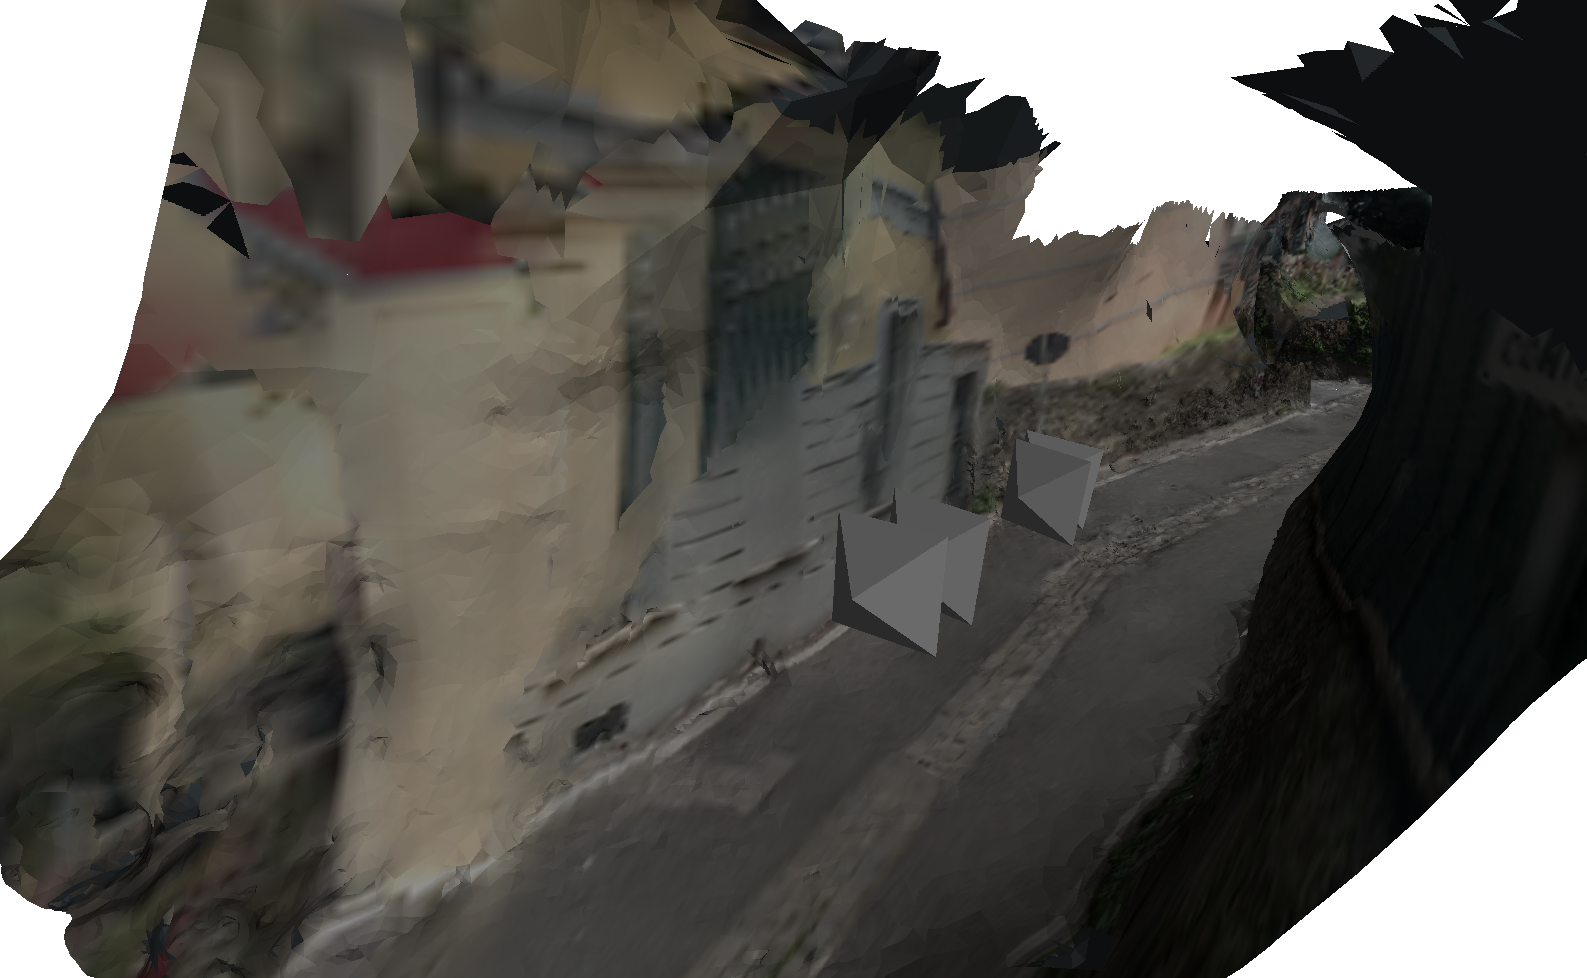
\includegraphics[width=0.48\textwidth]{./img/ch-further/snapshot01}&
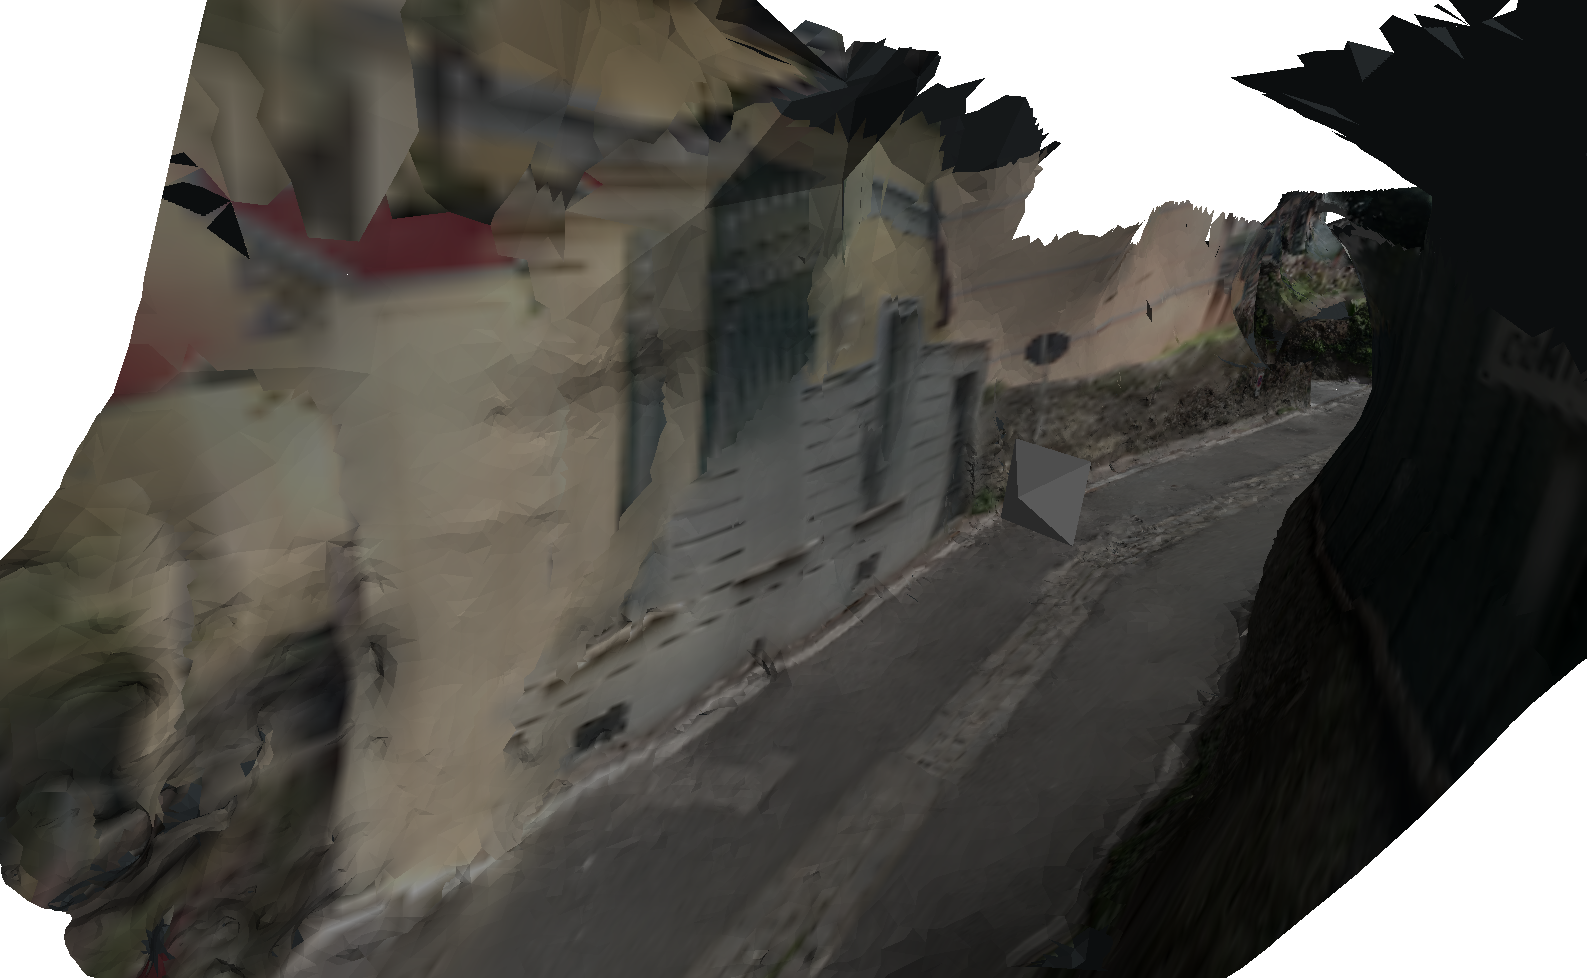
\includegraphics[width=0.48\textwidth]{./img/ch-further/02-bestImage02}\\
(a)&(b)\\
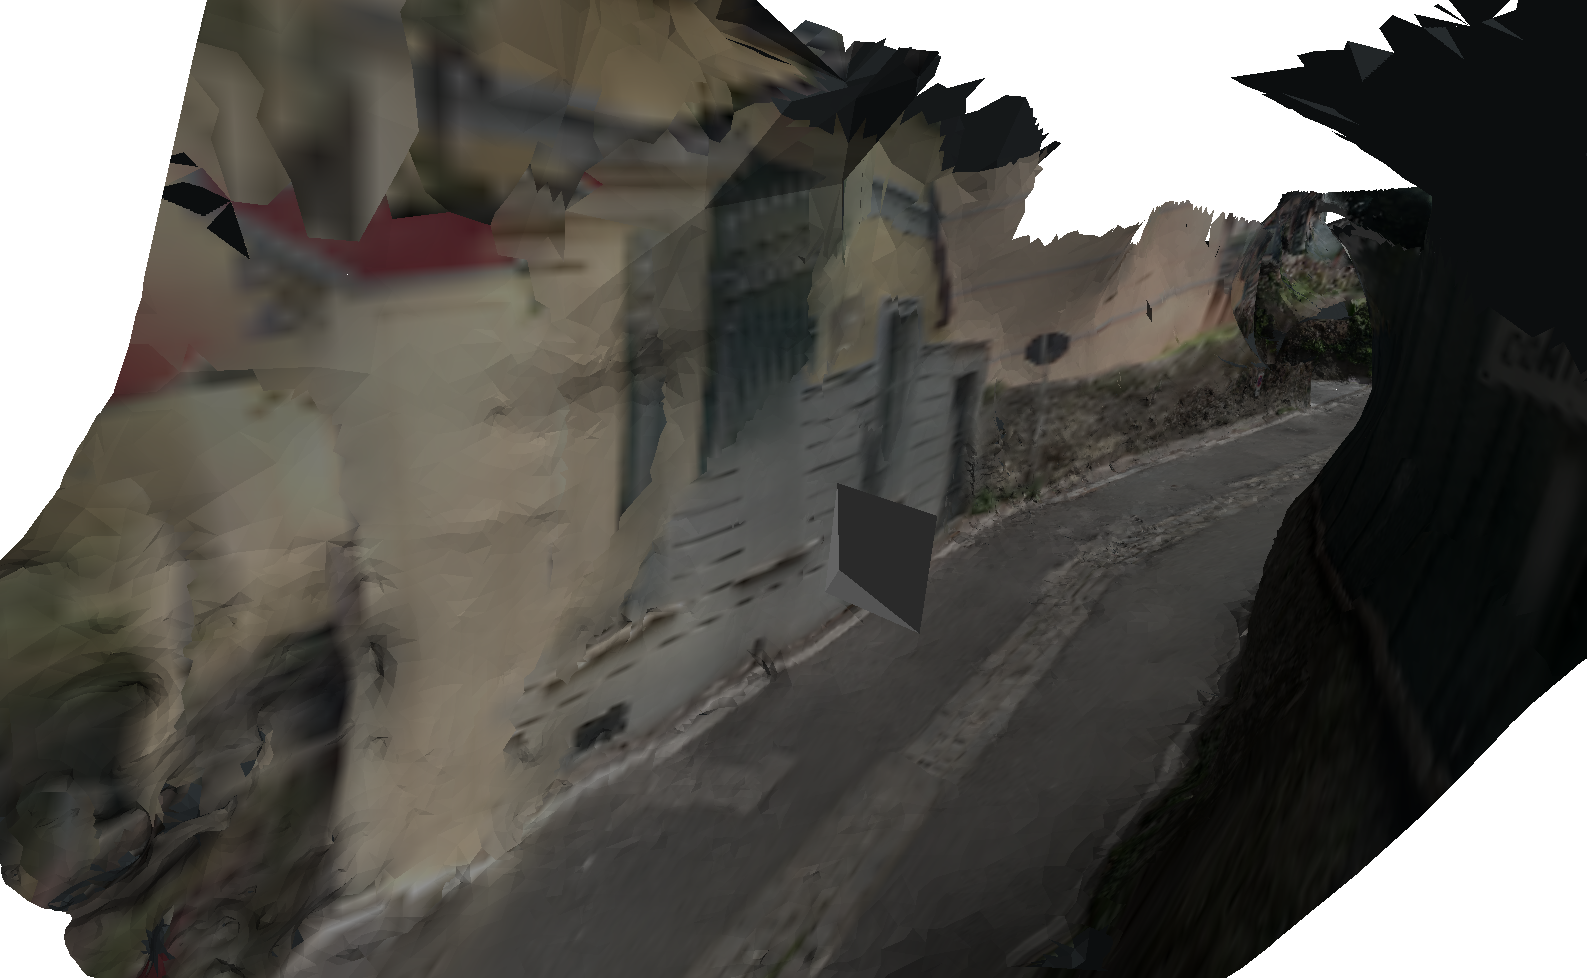
\includegraphics[width=0.48\textwidth]{./img/ch-further/03-localize07}&
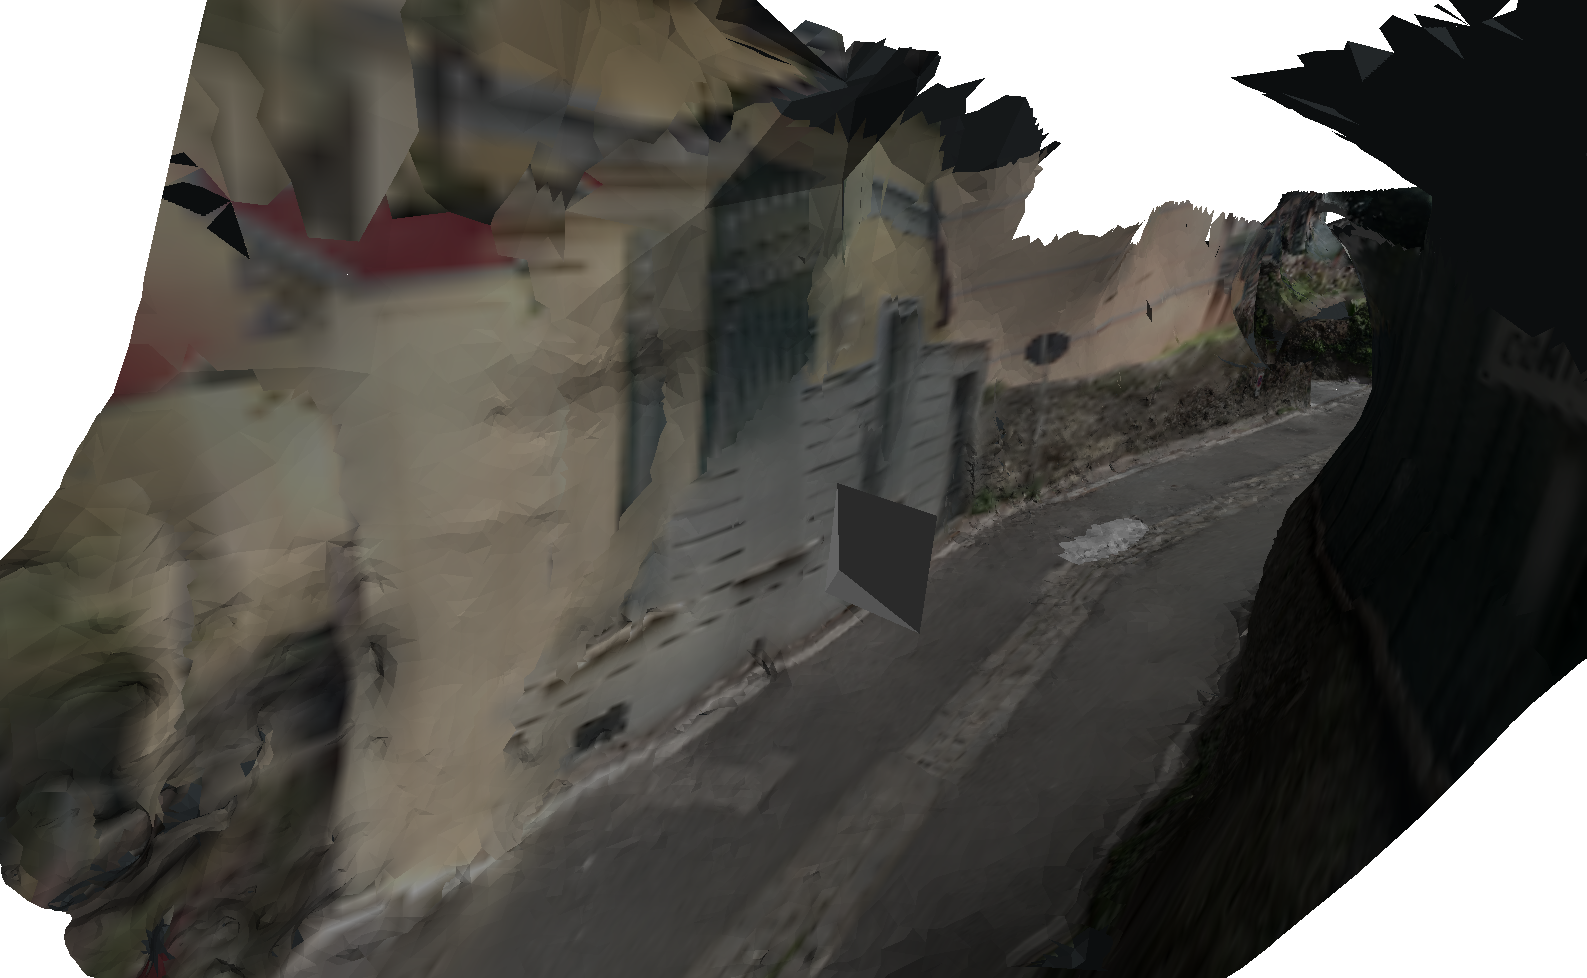
\includegraphics[width=0.48\textwidth]{./img/ch-further/04-projection08}\\
(c)&(d)\\
\end{tabular}
\caption{Localization of a camera and \emph{bas state region} projection}
\label{fig:mep_localize}
\end{figure}



\begin{figure}[t]
\centering
\begin{tabular}{cc}
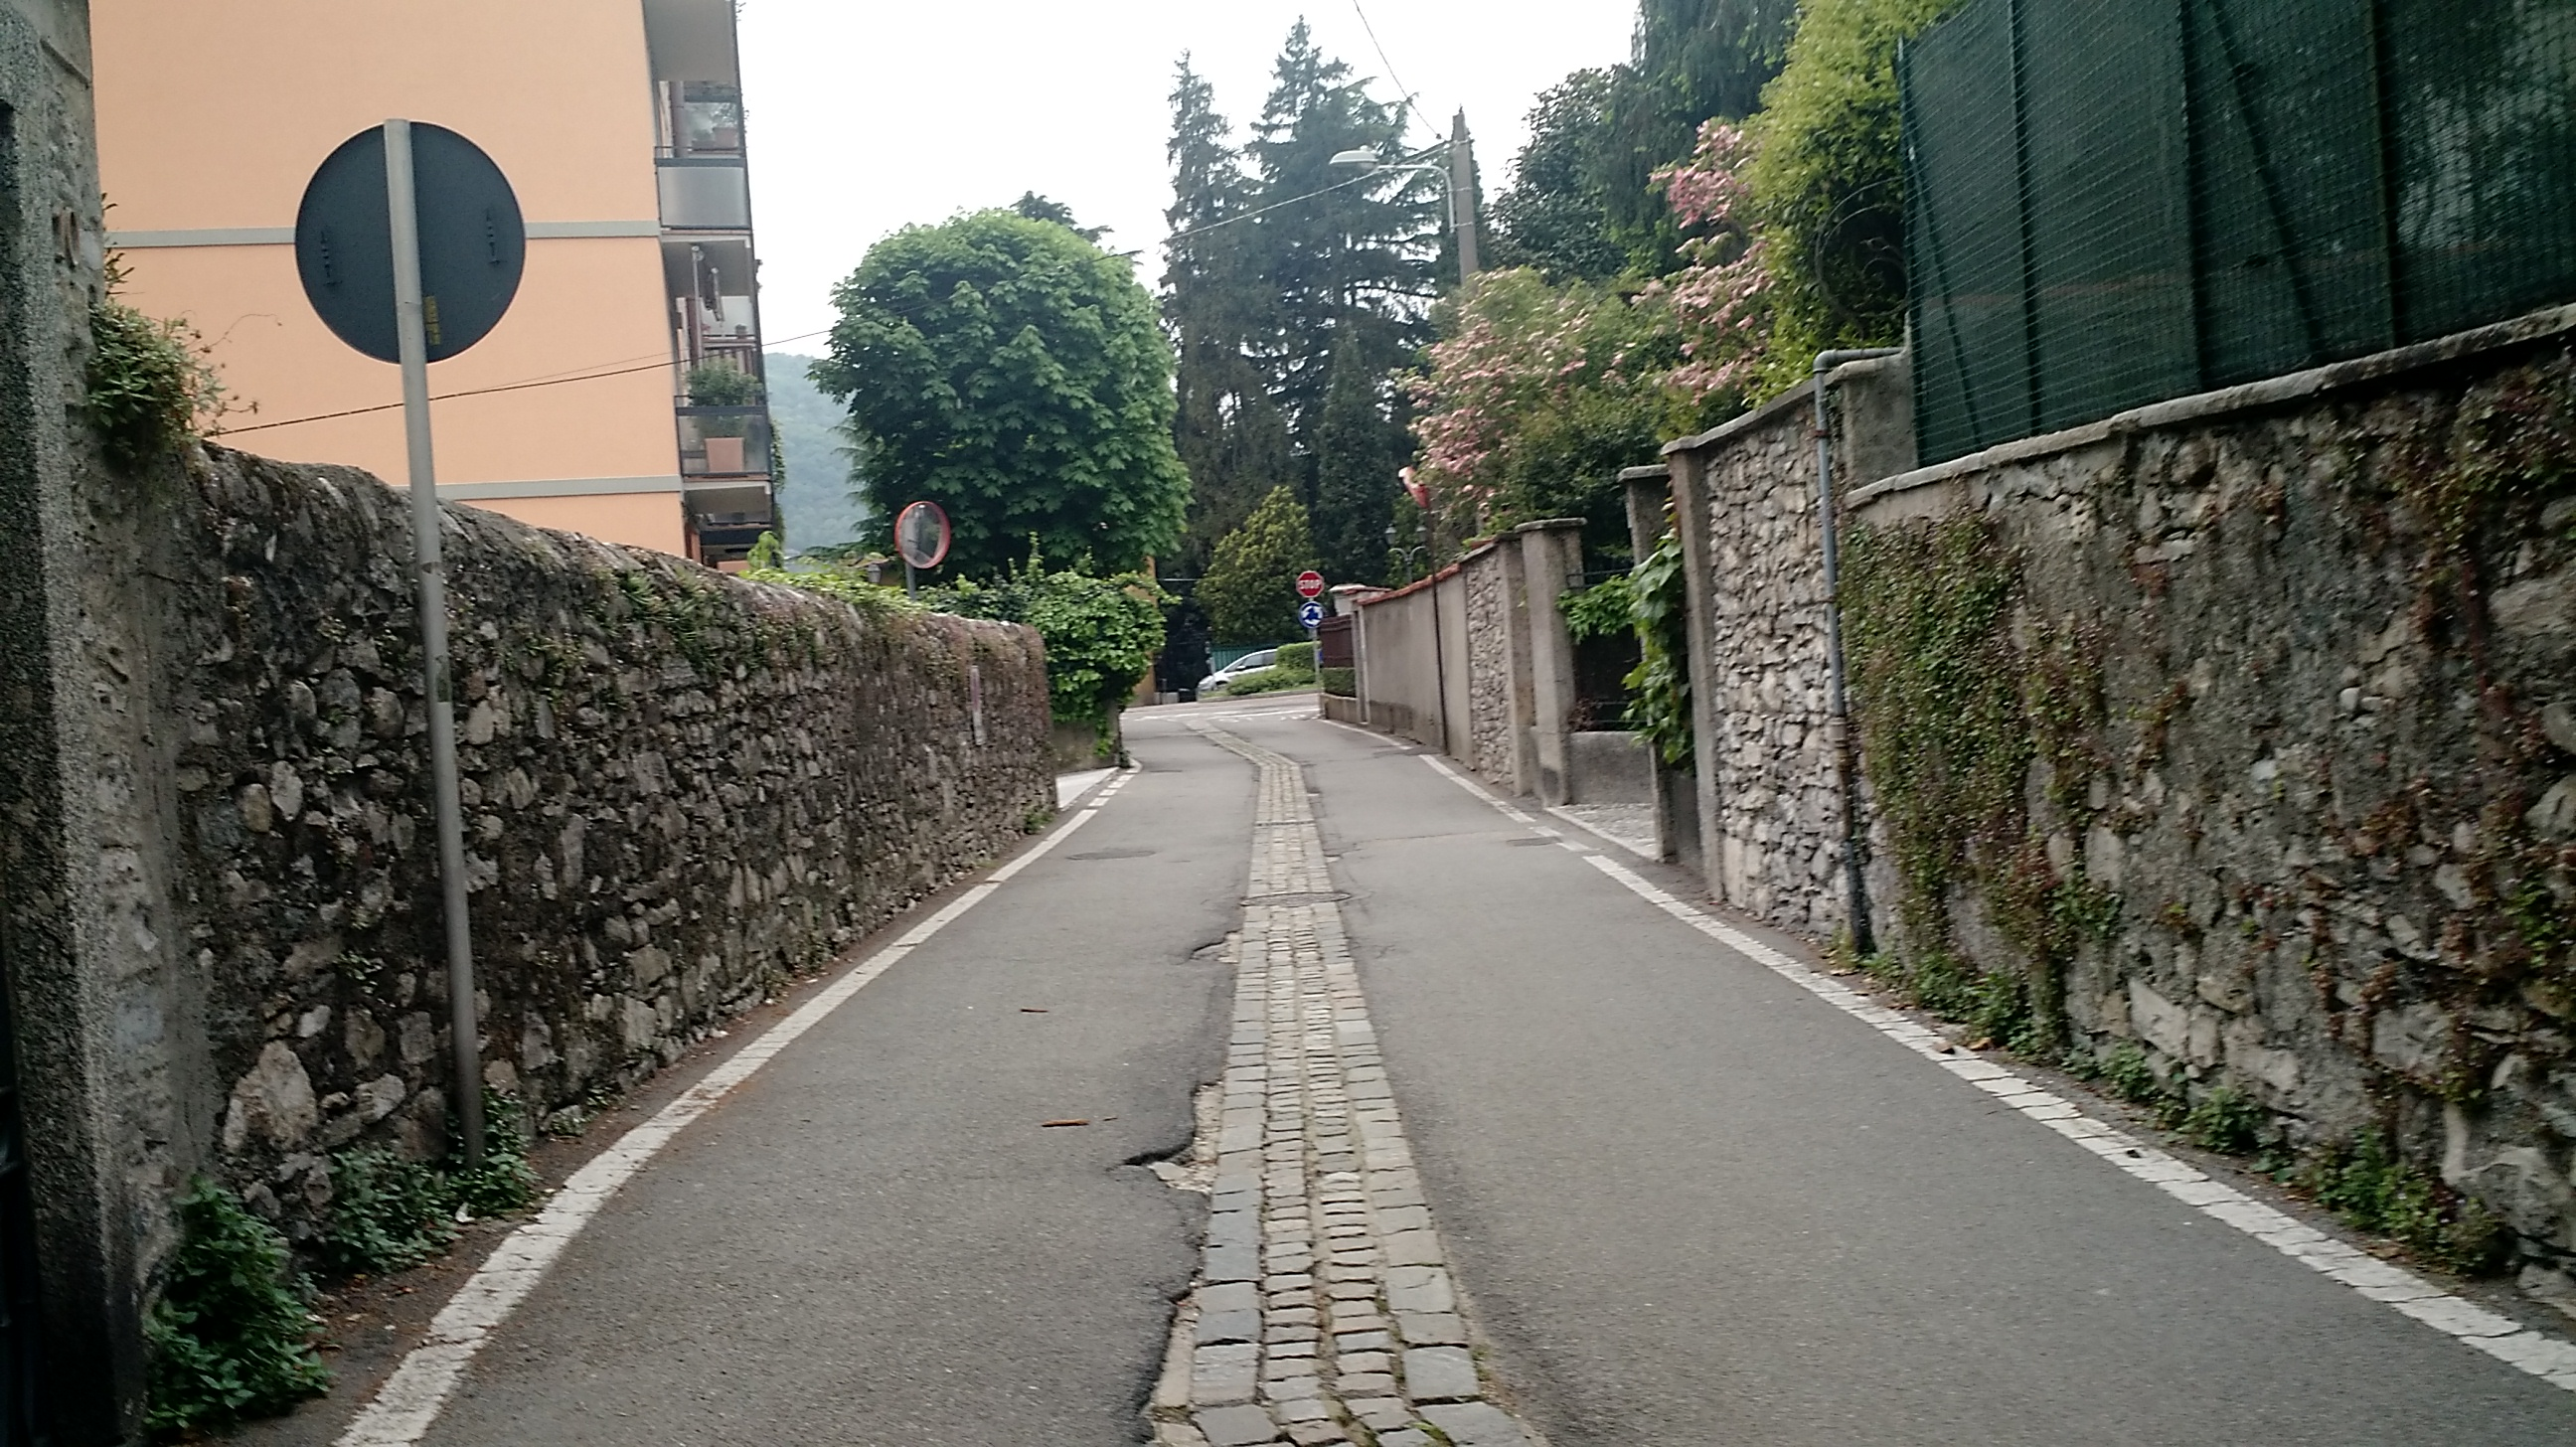
\includegraphics[width=0.55\textwidth]{./img/ch-further/1461225656475_MEP_IMAGE}&
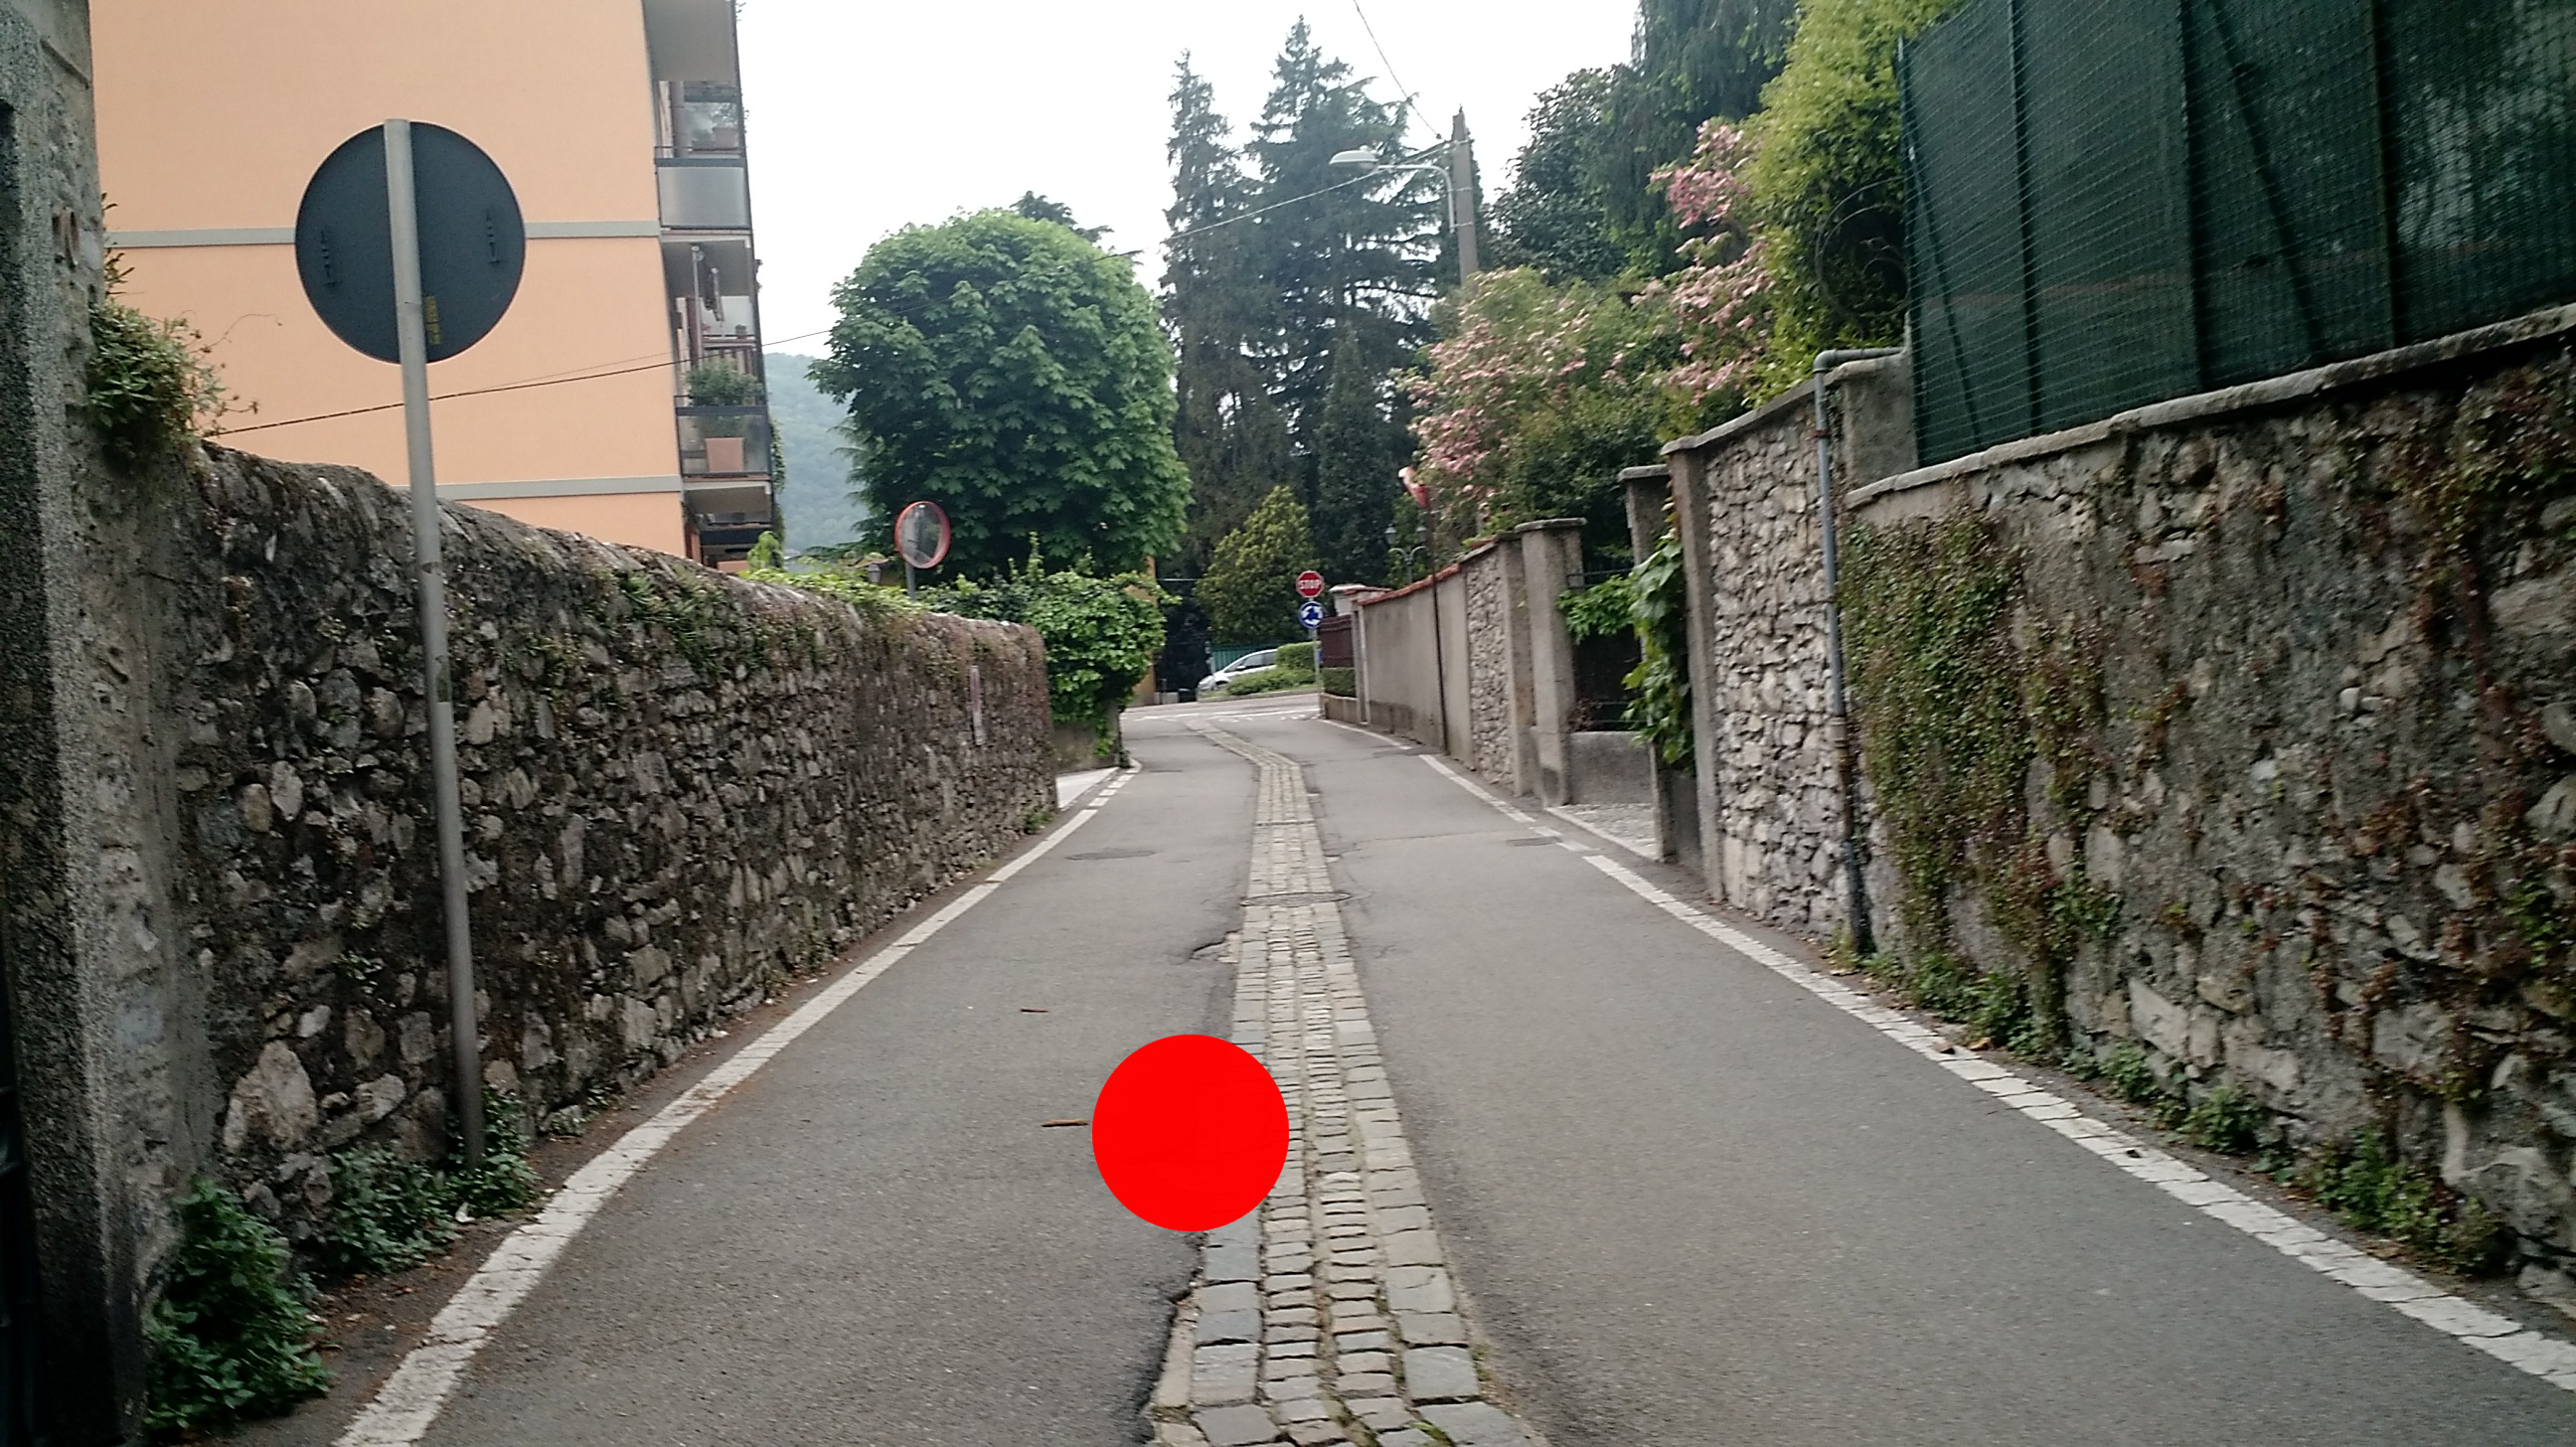
\includegraphics[width=0.55\textwidth]{./img/ch-further/1461225656475_MEP_IMAGE_with_mark}\\
(a)&(b)\\
\end{tabular}
\caption{Query image with the red circle in correspondence of a \emph{bad state region}}
\label{fig:mep_project}
\end{figure}

